\documentclass[11pt, oneside]{article}   	% use "amsart" instead of "article" for AMSLaTeX format

\usepackage{geometry}                		% See geometry.pdf to learn the layout options. There are lots.
\geometry{letterpaper}                   		% ... or a4paper or a5paper or ... 
\usepackage{graphicx}				% Use pdf, png, jpg, or eps§ with pdflatex; use eps in DVI mode
								% TeX will automatically convert eps --> pdf in pdflatex		
\usepackage[english]{babel}
\usepackage[QX]{fontenc}
\usepackage{amssymb}
\usepackage{subfig}
\usepackage[absolute,overlay]{textpos}
\usepackage{colortbl}
\usepackage{multirow}
\usepackage{booktabs}
\usepackage[framemethod=TikZ]{mdframed}
\usepackage{bbding}
\usepackage{listings}

\usepackage{tikz}
\usetikzlibrary{calc}

% tikzmark command, for shading over items
\newcommand{\tikzmark}[1]{\tikz[overlay,remember picture] \node (#1) {};}

\newtheorem{algorithm}{Algorithm}

\usepackage{setspace}
\setlength{\TPHorizModule}{1mm}
\setlength{\TPVertModule}{1mm}

%% user's definition

\newcommand{\minitab}[2][c]{\begin{tabular}{#1}#2\end{tabular}}

\newcommand{\tol}{\mbox{TOL}}
\newcommand{\sK}{\mathcal{K}}
\newcommand{\sN}{\mathcal{N}}
\newcommand{\sC}{\mathcal{C}}
\newcommand{\sF}{\mathcal{F}}
\newcommand{\sG}{\mathcal{G}}
\newcommand{\sT}{\mathcal{T}}
\newcommand{\sA}{\mathcal{A}}
\newcommand{\fA}{\mathfrak A}
\newcommand{\sP}{\mathcal{P}}
\newcommand{\sQ}{\mathcal{Q}}
\newcommand{\sH}{\mathcal{H}}
\newcommand{\sR}{\mathcal{R}}
\newcommand{\sE}{\mathcal{E}}
\newcommand{\sV}{\mathcal{V}}
\newcommand{\dK}{\mathbb{K}}
\newcommand{\dV}{\mathbb{V}}
\newcommand{\trno}[1]{\left|\!\left|\!\left| #1 \right|\!\right|\!\right|}
\newcommand{\tHs}{\tilde{H}^{s}}
\newcommand{\tHns}{H^{-s}}
\newcommand{\ltHs}{H_\Gamma^{s}}
\newcommand{\enorm}[1]{\trno{#1}}
\newcommand{\denorm}[1]{\trno{#1}_*}
\newcommand{\Hsnorm}[1]{\left\|#1\right\|_{\tHs(\Omega)}}
\newcommand{\dHsnorm}[1]{\left\|#1\right\|_{\tHns(\Omega)}}
\newcommand{\dHsw}[1]{\left\| #1 \right\|_{\tHns(\omega_z)}}

\newcommand{\IR}{\mathbb{R}}
\newcommand{\hR}{\widehat R}
\newcommand{\ang}[1]{\left<#1\right>}
\newcommand{\field}{\mathfrak F}
\newcommand{\ubar}{\overline{u}}
\newcommand{\Ubar}{\overline{U}}
\newcommand{\Fbar}{\overline{F}}
\newcommand{\sGbar}{\overline{\sG}}
\newcommand{\ds}{\displaystyle}
\newcommand{\hpsi}{\hat\psi_{\tau}}
\newcommand{\GT}{\left.\overline{\sG_h\psi_z}\right|_{\tau}}
\newcommand{\osc}{\text{\rm osc}}
\newcommand{\Dof}{\text{DOF}}

\newcommand{\bU}{\overline U}
\newcommand{\bu}{\overline u}
\newcommand{\bF}{\overline F}
\newcommand{\sbar}{\overline\Lambda}
\newcommand{\vu}{{\bf{u}}}
\newcommand{\vU}{{\mathbf{U}}}
\newcommand{\vv}{{\bf{v}}}
\newcommand{\vV}{{\mathbf{V}}}
\newcommand{\vF}{{\bf{F}}}
\newcommand{\vf}{{\bf{f}}}
\newcommand{\vg}{{\bf{g}}}
\newcommand{\vh}{{\bf{h}}}
\newcommand{\vI}{{\bf{I}}}
\newcommand{\vC}{{\bf{C}}}
\newcommand{\vX}{{\bf{X}}}
\newcommand{\vL}{{\bf{L}}}
\newcommand{\vW}{{\bf{W}}}
\newcommand{\vH}{{\bf{H}}}
\newcommand{\vR}{{\bf{R}}}

\DeclareMathOperator*{\diag}{diag}

\newcommand{\normV}[1]{\left\|#1\right\|_{\sV}}
\newcommand{\normdualV}[1]{\left\|#1\right\|_{\sV^*}}
\newcommand{\normH}[1]{\left\|#1\right\|_{\sH}}
\newcommand{\starS}{\mathfrak{S}}
\newcommand{\starI}{\mathfrak{I}}


\mdfdefinestyle{mystyle}{leftmargin=0.2cm, rightmargin=0.2cm, linecolor=blue, backgroundcolor=yellow!50, linecolor=blue, linewidth=1pt, roundcorner=5pt}

\mdfdefinestyle{mystyle1}{leftmargin=0.4cm, rightmargin=0.4cm, linecolor=blue, backgroundcolor=yellow!50, linecolor=blue, linewidth=1pt, roundcorner=5pt}

\mdfdefinestyle{mystyle2}{leftmargin=0.05cm, rightmargin=0.05cm, linecolor=blue, backgroundcolor=green!30, linewidth=1pt}

\mdfdefinestyle{mystyle3}{leftmargin=0.4cm, rightmargin=0.4cm, linecolor=red, topline=false, bottomline=false, linewidth=3pt}

\mdfdefinestyle{mystyle4}{leftmargin=0.2cm, linecolor=red, topline=false, bottomline=false, rightline=false, linewidth=4pt}

% Define the listings environment
\usepackage{listings}
\usepackage{textcomp}
\definecolor{listinggray}{gray}{0.95}
\definecolor{deepblue}{rgb}{0.1,0,0.7}
\definecolor{deepred}{rgb}{0.6,0,0}
\definecolor{deepgreen}{rgb}{0,0.5,0}

\usepackage[utf8]{inputenc}
\DeclareFixedFont{\ttb}{T1}{txtt}{bx}{n}{9} % for bold
\DeclareFixedFont{\ttm}{T1}{txtt}{m}{n}{9} % for normal

\lstset{
        columns=fixed,
        %extendedchars=true,
        frame=single,
        linewidth=0.95\linewidth,
        xleftmargin=18pt,
        numbers=left,
        numberstyle=\tiny\ttfamily,
        stepnumber=1,
        backgroundcolor=\color{listinggray},
	tabsize=4,
	language=python,
	basicstyle=\tiny,
     	keywordstyle=\color{deepblue},
	emph={MyClass,__init__},          
	emphstyle=\color{deepred},    
	stringstyle=\color{red},
	commentstyle=\color{deepgreen},
	showstringspaces=false,
	literate = {-}{-}1, % <------ trick!
}

%%% Always I forget this so I created some aliases
\def\ContinueLineNumber{\lstset{firstnumber=last}}
%\def\StartLineAt#1{\lstset{firstnumber=#1}}
%\let\numberLineAt\StartLineAt
 
%%%%%%%%%%%%%%%%%%%%%%%%%%%%%%%%%%%%%%%%%%%%
\title{A Quick Survey on Deep Learning Engines}
%%%%%%%%%%%%%%%%%%%%%%%%%%%%%%%%%%%%%%%%%%%%

\author{Chensong Zhang}

\date{April 27, 2017}

%%%%%%%%%%%%%%%%%%%%%%%%%%%%%%%%%%%%%%%%%%%%
\begin{document} % Start your content from here ...
%%%%%%%%%%%%%%%%%%%%%%%%%%%%%%%%%%%%%%%%%%%%

\maketitle


\section{Introduction}\label{sec:intro}

%%%

%%%
\subsection{Background}
%%%

Unlike traditional numerical simulation, ``ML gives computers the ability to learn without being explicitly programmed''. As a research field, ML explores the study and construction of algorithms that can {learn} from and {make predictions} on {data}. General Tasks of ML include:

\begin{itemize}

\item Classification: Inputs are divided into two or more classes, and the learner must produce a model that assigns unseen inputs to one or more of these classes

\item Regression: Similar to classification, but the outputs are continuous

\item Clustering: Inputs are divided into several groups (Unlike in classification, the groups are not known beforehand, making this an unsupervised task)

\item Density estimation, dimension reduction, ...

\end{itemize}

There are many machine learning engines available; see the following picture:
\begin{figure}[htbp] %  figure placement: here, top, bottom, or page
   \centering
   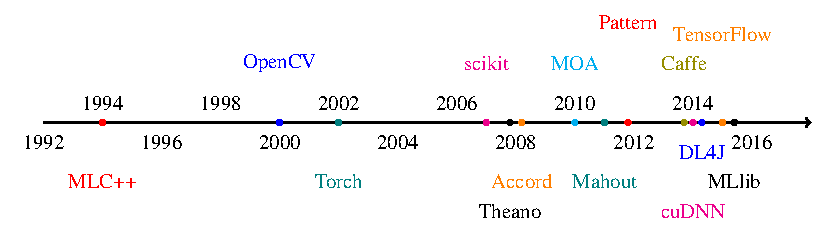
\includegraphics[width=\linewidth]{figures/ML.pdf}
   \caption{Refer to Tour of TensorFlow, by Peter Goldsborough, arXiv, 2016}
\end{figure}

Besides the packages mentioned in the above figure, there are a few {other worth-noting ML (DL) packages:}
\begin{itemize}\setlength\itemsep{0.25em}
	\item PyTorch (still in {beta} stage)
	\item Theano (Lasagne/Keras): Slow in graph compilation
	\item MXNet (DMLC): First released on Jan 2015, scalable distributed computing
	\item CNTK/DMTK (Microsoft): First released on April 2015
		\begin{itemize}
		\item[-] Windows/Linux, no official OS X support thought
		\item[-] C++/Python front-end
		\end{itemize}
	\item Neon (Nervana \& Intel): First released on May 2015, professional support
	\item Caffe2 (Google, Facebook, ...): Release on late 2016
	\item Digits (Nvidia, powered by Caffe): Web interface
\end{itemize}

%%%
\subsection{DL engines}
%%%

In this talk, we shall talk about the most popular DL engines that are freely available. So what do we want for a software package which are suitable for deep learning research?
\begin{itemize}
\item Easy for debugging (with good {documentation}, {support}, and active community)
\item Good flexibility
	\begin{itemize}
	\item[-] Easy to add new tasks
	\item[-] Easy to build new network structures
	\end{itemize}
\item Good performance and scalability
	\begin{itemize}
	\item[-] Multicore CPU
	\item[-] {Single} or {multiple} GPU(s)
	\item[-] Cluster
	\end{itemize}
\end{itemize}
%
Among dozens of available software packages, we mainly look at Torch, Caffe, TensorFlow, and MXNet; see Table~\ref{tab:comparison} for the basic information about these four packages. 
%
\renewcommand{\multirowsetup}{\centering} 
\begin{table}[htbp]
\begin{center}
\begin{tabular}{|c|c|c|c|c|c|} \hline
Viewpoint &Torch       &Caffe   & TensorFlow  & MXNet \\ \hline
\multirow{2}{4em}{First \\Released} & \multirow{2}{3em}{2002} & \multirow{2}{3em}{2013} & \multirow{2}{3em}{2015} & \multirow{2}{3em}{2015} \\
&   &    & &      \\ \hline
 \multirow{3}{4em}{Main \\Developers}
 & Facebook,        &\multirow{3}{5em}{BAIR \\ BVLC}  &\multirow{3}{3em}{Google} &\multirow{3}{*}{DMLC}   \\ 
 &Twitter,            & & &    \\
 &Google, ...       & & &  \\ \hline 
\multirow{2}{4em}{ Core \\Languages}     
& \multirow{2}{3em}{ C/Lua }      
&\multirow{2}{4em}{ C++}
&\multirow{2}{4em}{ C++ \\Python}
&\multirow{2}{6em}{ C++}  \\ 
&   &    & &      \\ \hline
\multirow{2}{4em} {Supported \\Interface }    
& \multirow{2}{3em}{ Lua }      
&\multirow{2}{5.5em}{ C++/Python \\ Matlab}
&\multirow{2}{6.2em}{ {Python}/C++/{R} \\ Java/Go/...}  
&\multirow{2}{6.2em}{ C++/{Python}/{R} \\ Matlab/Julia/...}\\  
&   &    & &      \\ \hline           
 \multirow{2}{4em}{ License }     
& \multirow{2}{3em}{BSD}      
&\multirow{2}{4em}{BSD}
&\multirow{2}{4em}{Apache}
&\multirow{2}{6em}{Apache}  \\ 
&   &    & &      \\ \hline
  \multirow{2}{4.5em}{Pretrained \\ Models}      
  &  \multirow{2}{4em} {Yes}      
  &  \multirow{2}{4em}{Yes}                             
  &  \multirow{2}{4em}{No}                   
  &  \multirow{2}{4em}{Yes}\\ 
  &  &   &   & \\ \hline
\multirow{2}{4.5em}{High-level \\ Support}     
& \multirow{2}{*}{Good}      
&\multirow{2}{*}{ Good}
&\multirow{2}{*}{ Good}
&\multirow{2}{*}{ Good}  \\ 
&   &    & &      \\ \hline
 \multirow{2}{4em}{Low-level \\ Operators}
 &\multirow{2}{4em}{Good}
 &\multirow{2}{*}{Good }     
 &\multirow{2}{*}{Fairly good}
 &\multirow{2}{*}{Increasing fast}\\ 
 &       &    &  &  \\ \hline 
\multirow{2}{4em} {Speed \\ One-GPU }    
& \multirow{2}{*}{ Great }      
&\multirow{2}{*}{Great} 
&\multirow{2}{*}{Good}
&\multirow{2}{*}{Good} \\  
&   &    & &      \\ \hline          
\multirow{2}{5em} {Memory \\ Management}    
& \multirow{2}{*}{ Great }      
&\multirow{2}{*}{Great}
&\multirow{2}{*}{{Not so good}}
&\multirow{2}{*}{ Excellent}  \\  
&   &    & &      \\ \hline            
\multirow{2}{3.5em} {Parallel \\ Support}    
& \multirow{2}{5.em}{Multi-GPU}      
&\multirow{2}{5.em}{Multi-GPU}
&\multirow{2}{5.em}{{Multi-GPU}}
&\multirow{2}{5em}{Distributed} \\  
&   &    & &      \\ \hline            
\multirow{2}{3.5em} {Coding \\ Style}    
& \multirow{2}{5.em}{Imperative}      
&\multirow{2}{5.em}{Declarative}
&\multirow{2}{5.em}{Declarative} 
&\multirow{2}{5em}{Mixed} \\  
&   &    & &      \\ \hline
\multirow{2}{3.5em} {GitHub \\ Watching}    
& \multirow{2}{5.em}{649/268}      
&\multirow{2}{5.em}{1856}
&\multirow{2}{5.em}{4939} 
&\multirow{2}{5em}{887} \\  
&   &    & &      \\ \hline
\end{tabular}
\end{center}
\caption{Basic information on popular DL engines}\label{tab:comparison}
\end{table}%

%%%

\section{Comparison}\label{sec:numer}

%%%
\subsection{Test setting}
%%%

In order to compare performance of these software packages on CPU and GPU platforms, we look at the recent numerical study carried out in
\begin{center}
{\color{red}
Benchmarking State-of-the-Art Deep Learning Software Tools, by S.-H. Shi, et al., arXiv, 2017}
\end{center}
In this paper, different network models are tested on several consumer-class computing platforms; see Figures~\ref{fig:hardware} and \ref{fig:model}

\begin{figure}[htbp]\centering
	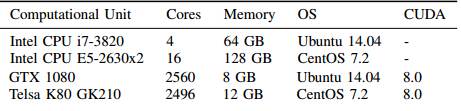
\includegraphics[width=\linewidth]{figures/platforms.png} 
	\caption{The experimental hardware settings for numerical tests}\label{fig:hardware}
\end{figure}
%
\begin{figure}[htbp]\centering
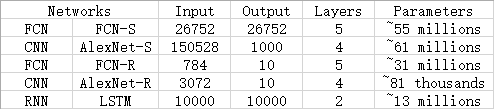
\includegraphics[width=\linewidth]{figures/models.png} 
\caption{The experimental setup of neural networks for synthetic and real data}\label{fig:model}
\end{figure}
	
%%%

\begin{itemize}

\item A large fully-connected neural network ({FCN-S}) with around 55 million parameters is used to evaluate the performance of FCN;

\item The classical AlexNet ({AlexNet-S}) is used as an representative of CNN;

\item A smaller FCN ({FCN-R}) is constructed for MNIST data set;

\item An AlexNet ({AlexNet-R}) architecture is used for Cifar10 data set;

\item For RNNs, considering that the main computation complexity is related to the length of input sequence, 2 LSTM layers with input length of 32.

\end{itemize}
	
%%%
\subsection{CPU tests}
%%%

From the numerical results on CPUs, we have the following observations:
\begin{itemize}
\item CNTK/Torch/Caffe have similar CPU performance
\item TensorFlow has excellent scalability
\item All engines have good CPU performance
\item TensorFlow has good scalability but considerably slower
\item Caffe has best CNN performance as promised
\item MXNet does not scale well for this test
\item Good scalability of TensorFlow kicks in 
\item Caffe does not scale well on multicore CPUs
\item Pay more attention to CNTK in the future
\item Caffe/MXNet does not support LSTM on CPUs
\end{itemize}

\begin{figure}[htbp] 
	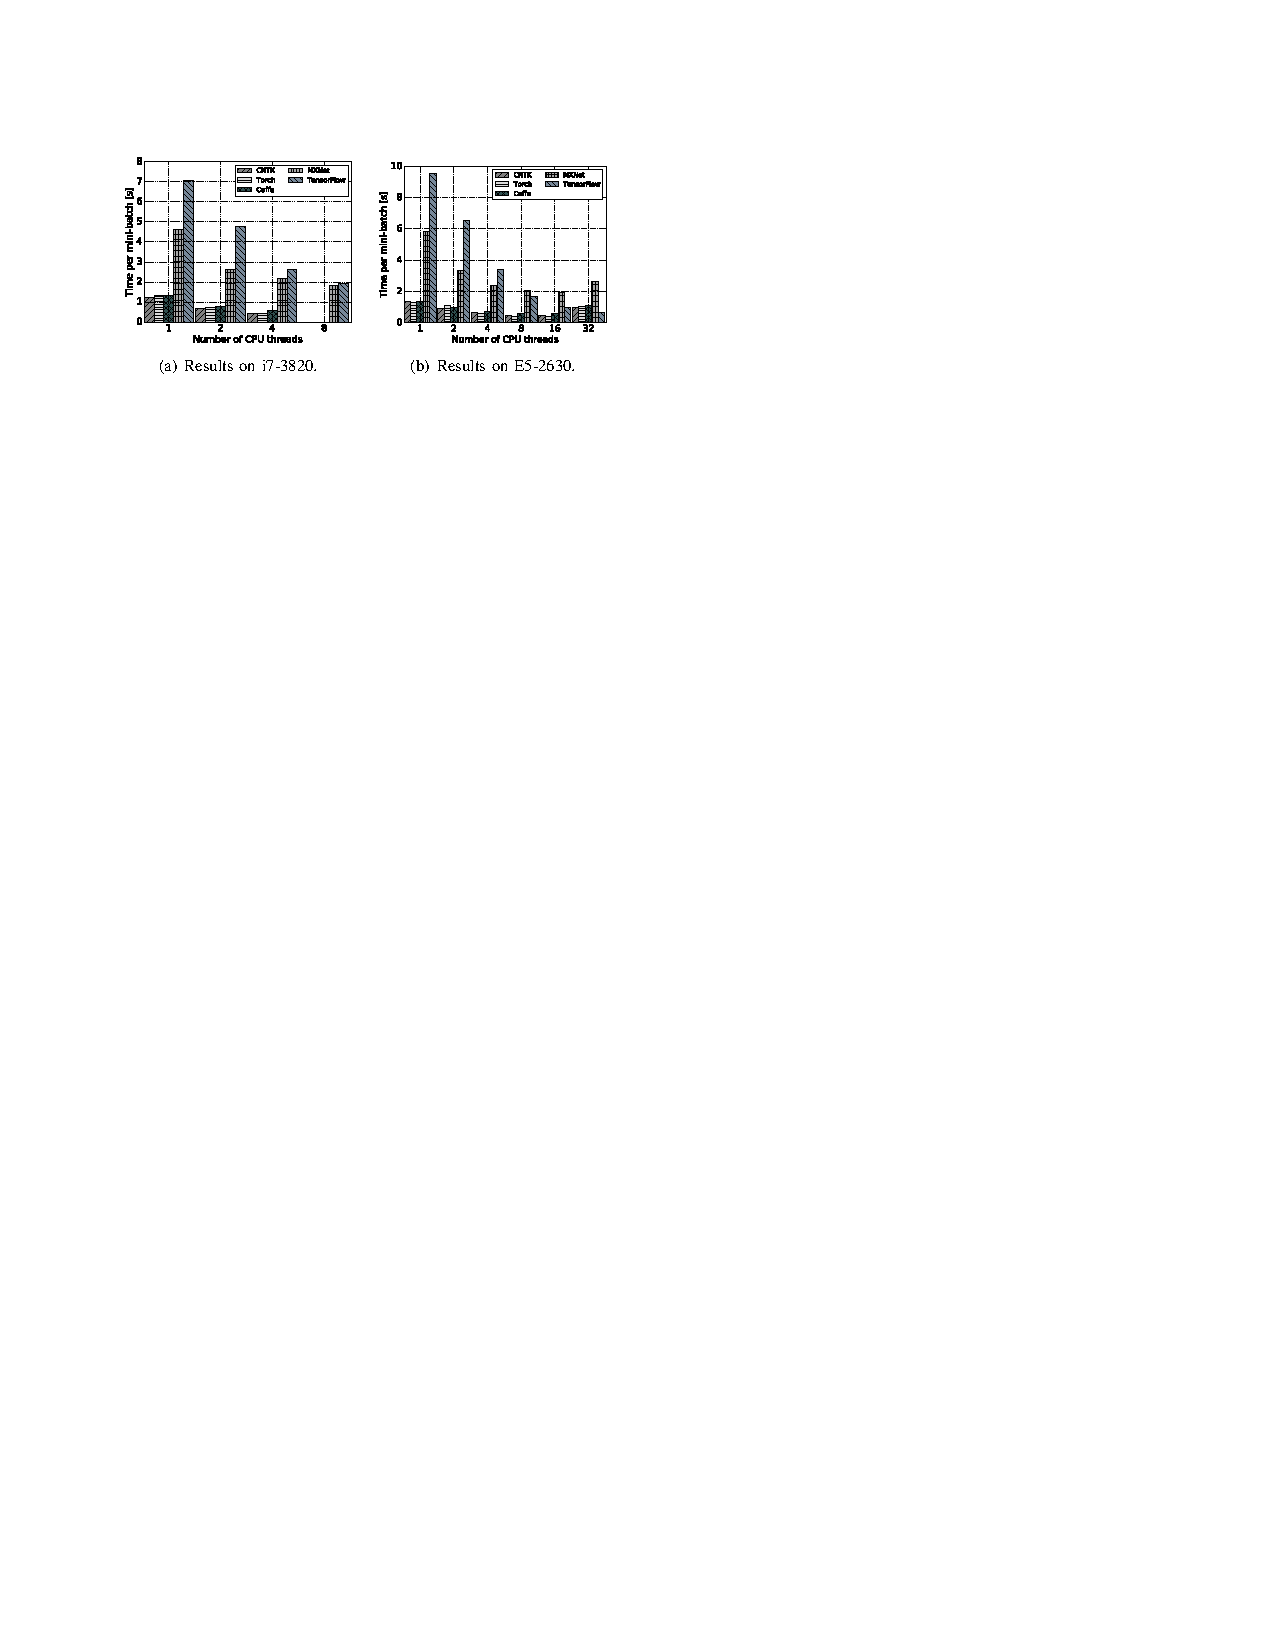
\includegraphics[width=\linewidth]{figures/FCN-S1.pdf} 
	\caption{FCN-S performance on CPU platform with a mini-batch size of 64}
\end{figure}
%
\begin{figure}[htbp] 
	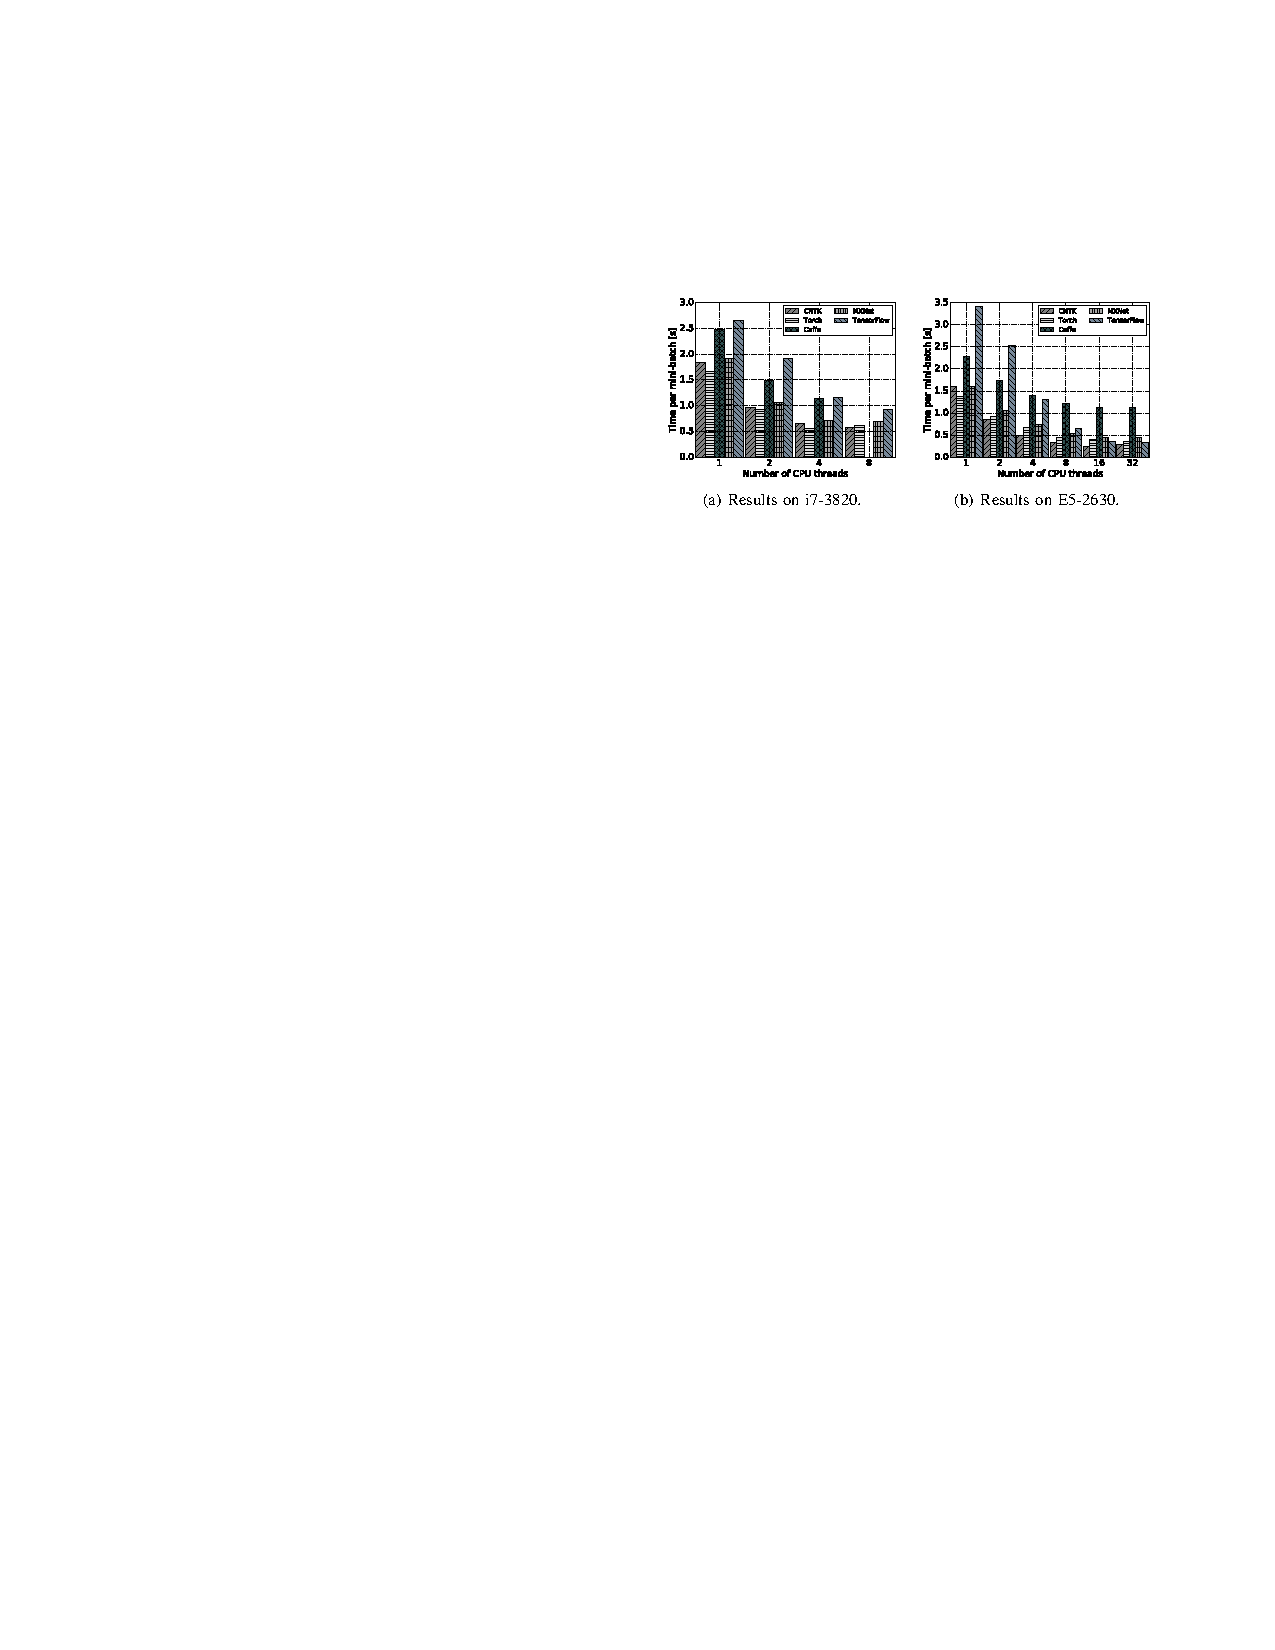
\includegraphics[width=\linewidth]{figures/FCN-R1.pdf} 
	\caption{The FCN-R performance on CPU platform with a mini-batch size of 1024}
\end{figure}
%
\begin{figure}[htbp] 
	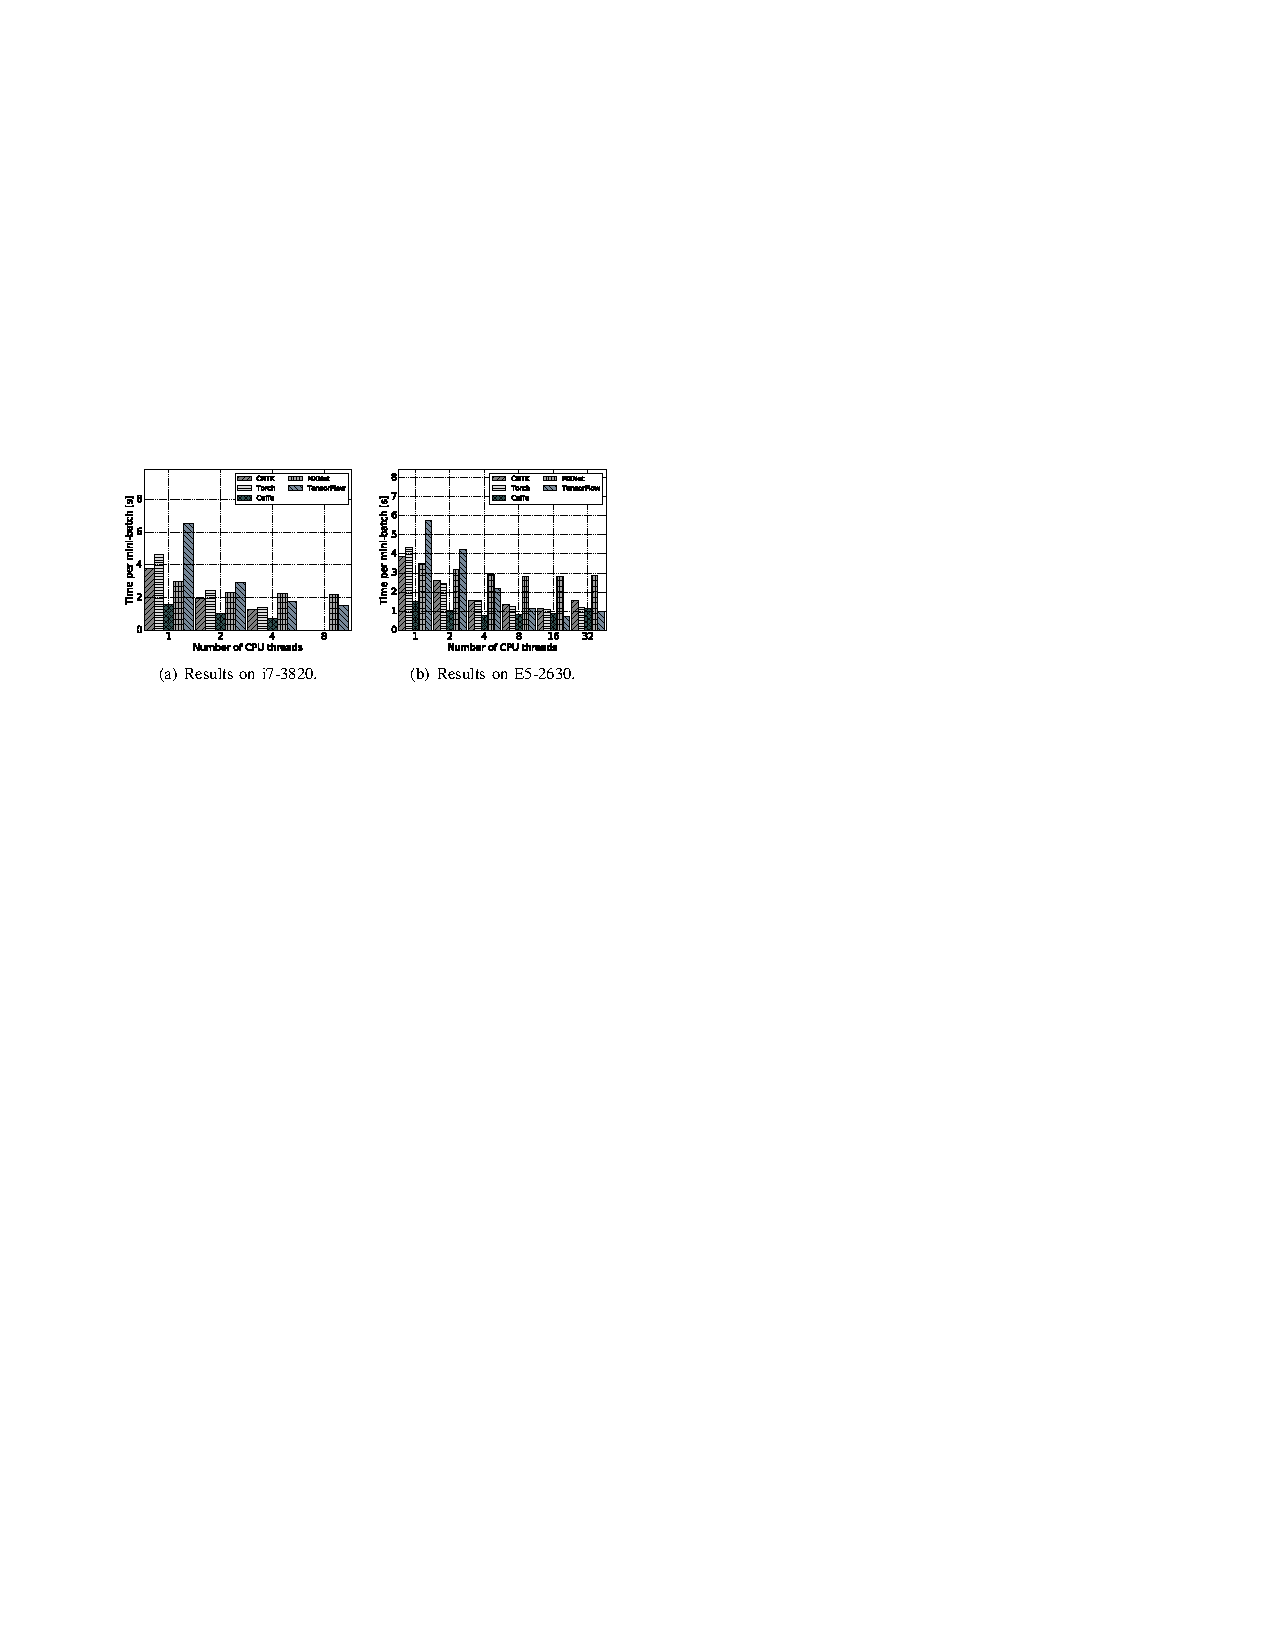
\includegraphics[width=\linewidth]{figures/AlexNet-S1.pdf} 
	\caption{AlexNet-S performance on CPU platform with a mini-batch size of 16}
\end{figure}
%
\begin{figure}[htbp] 
	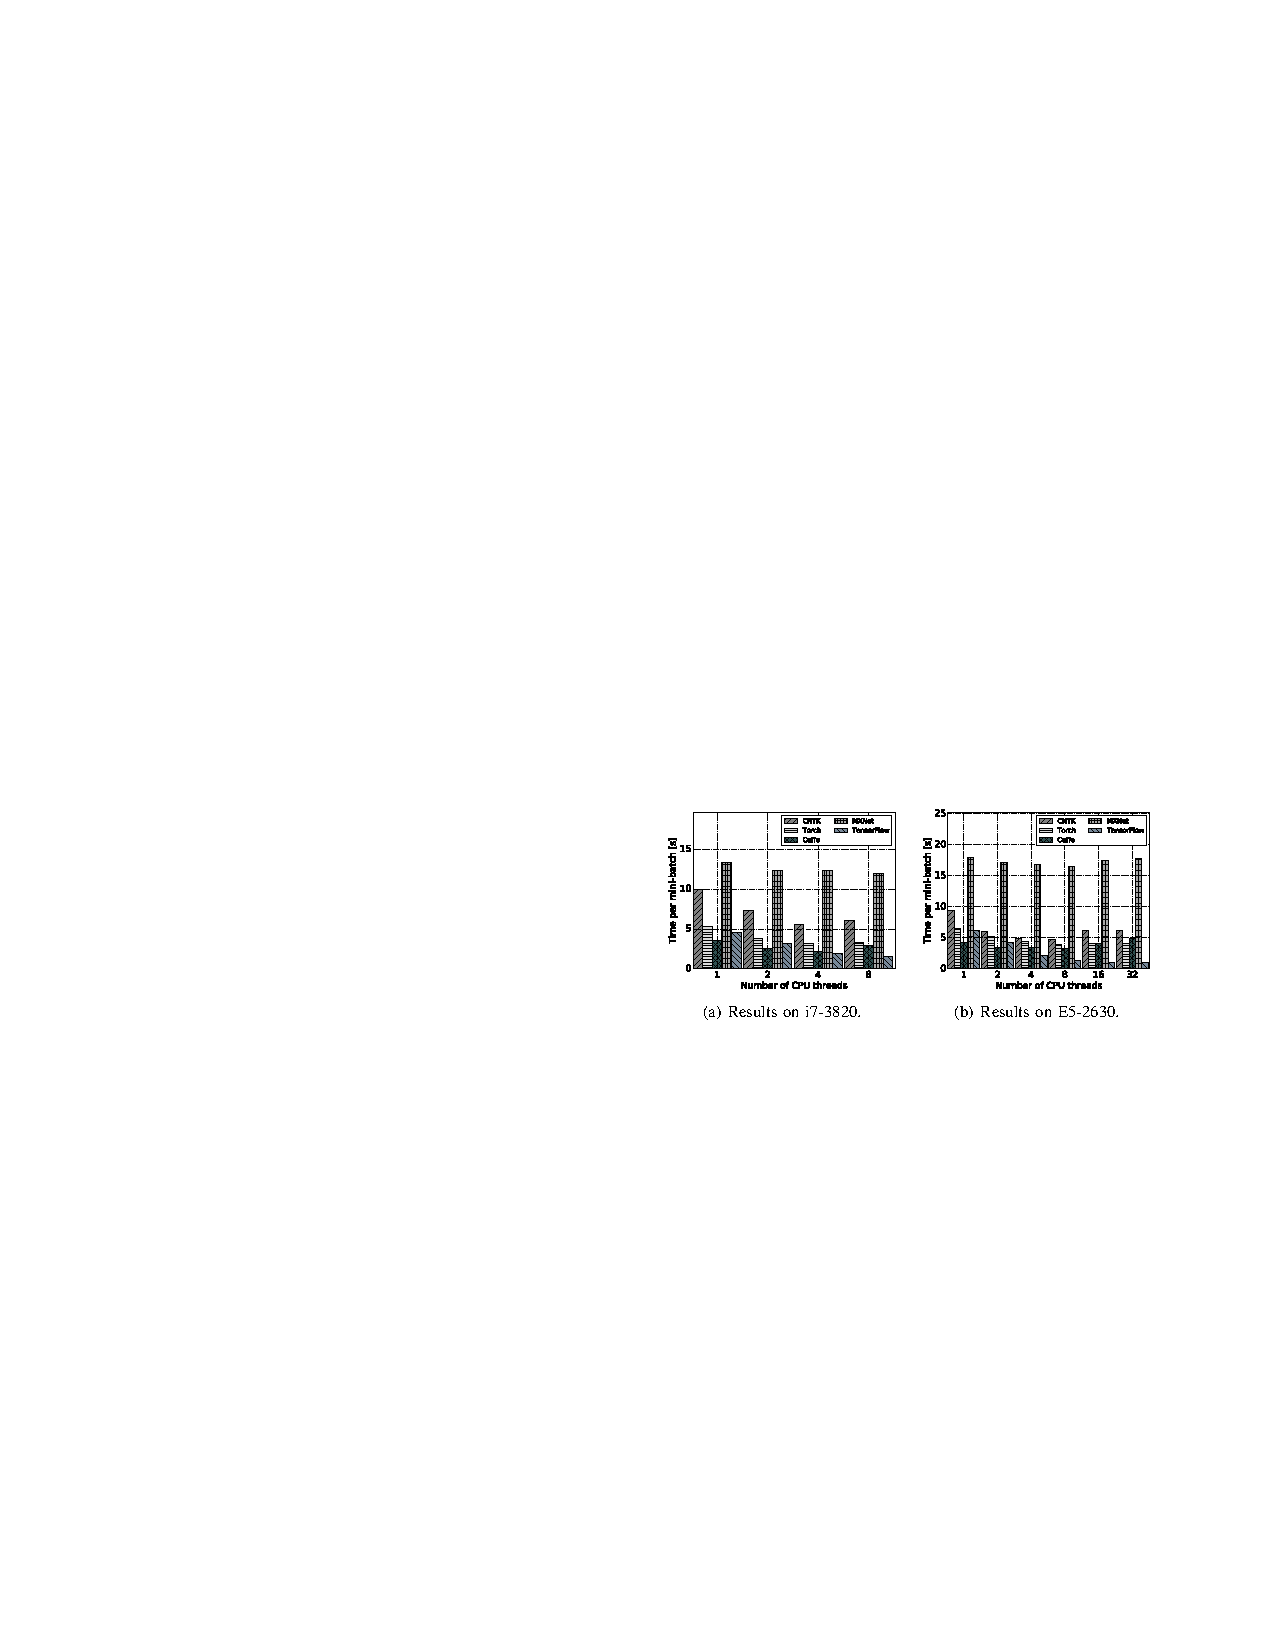
\includegraphics[width=\linewidth]{figures/AlexNet-R1.pdf} 
	\caption{AlexNet-R performance on CPU platform with a mini-batch size of 1024}
\end{figure}
%
\begin{figure}[htbp] 
	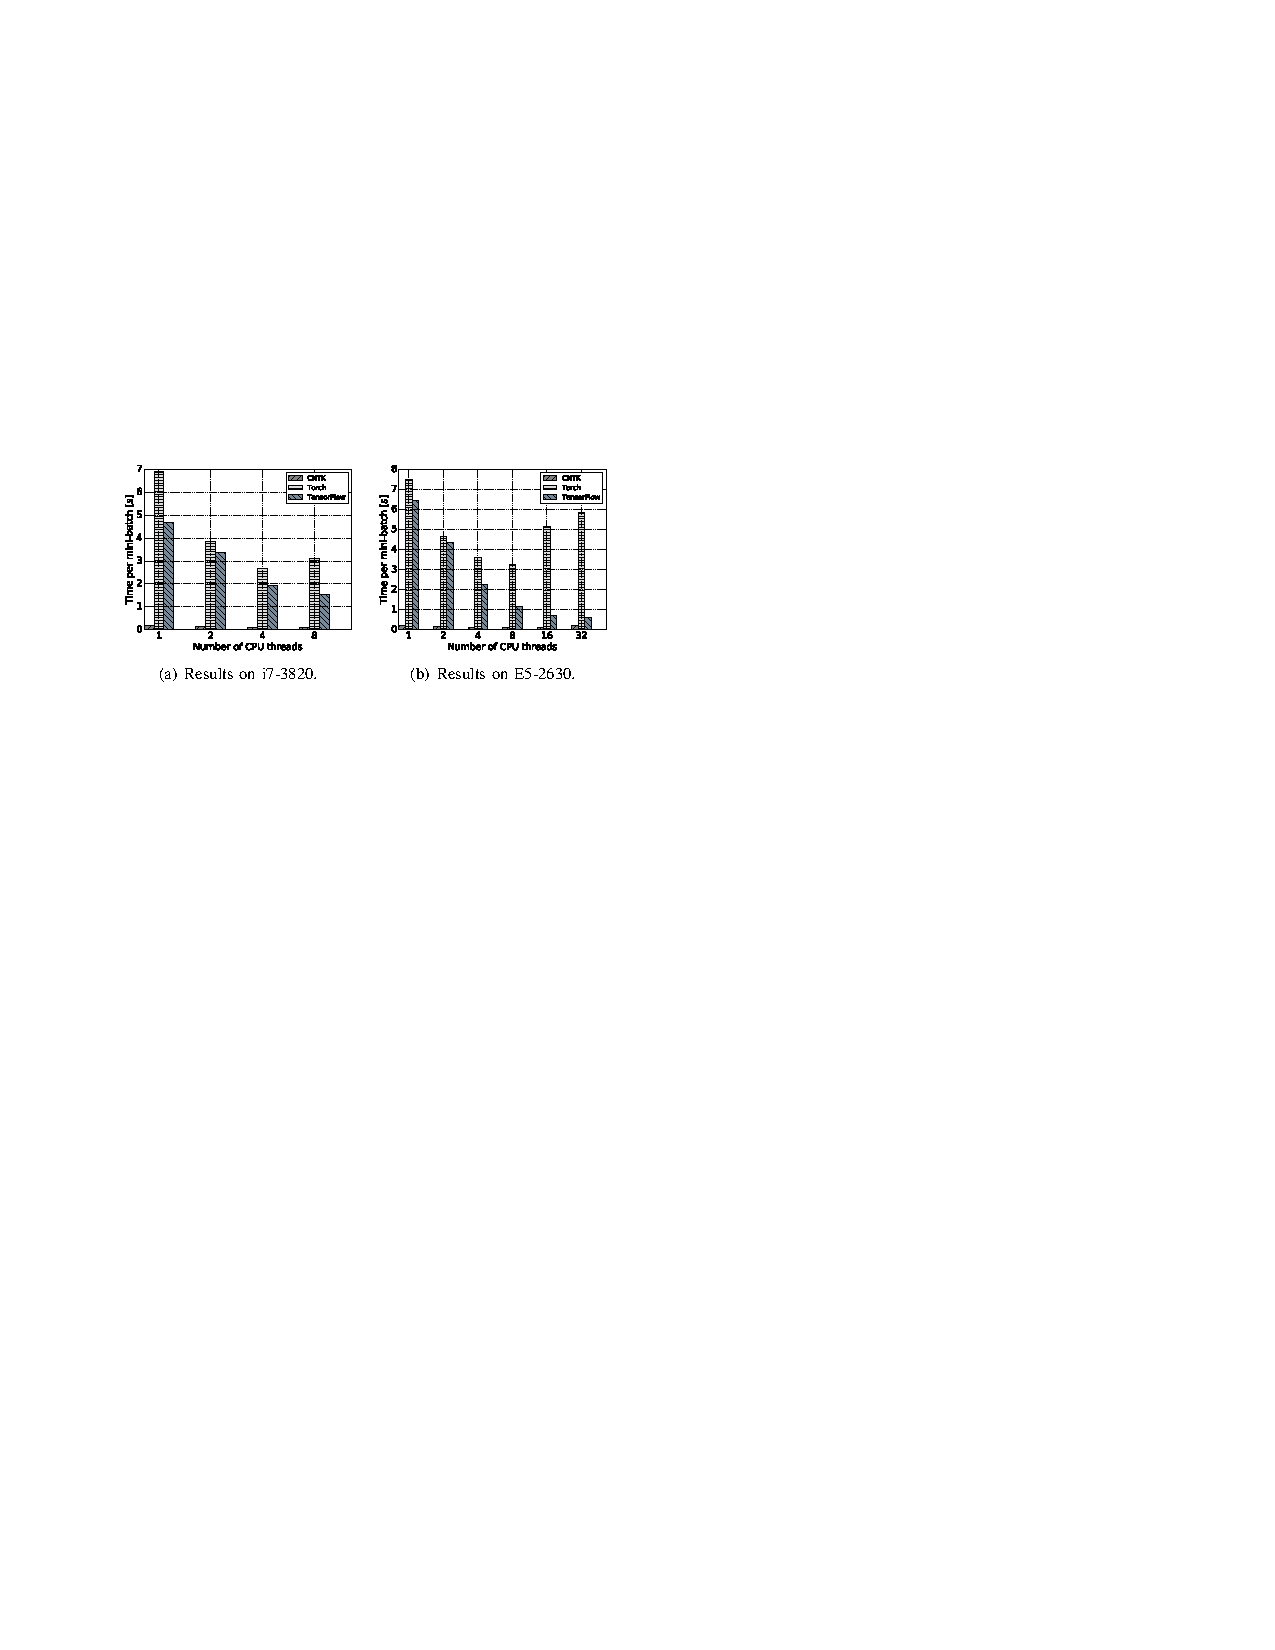
\includegraphics[width=\linewidth]{figures/LSTM1.pdf} 
	\caption{LSTM performance on CPU platform with a mini-batch size of 256}
\end{figure}

%%%
\subsection{GPU tests}
%%%

From the numerical results on GPUs, we have the following observations:
\begin{itemize}
\item CNTK/Torch/Caffe out-perform the others
\item All packages have similar performance
\item MXNet out-perform the others for CNN on GPUs
\item TensorFlow does not have good GPU performance in general
\item CNTK has excellent RNN performance both on CPU and GPU
\item Multi-GPU can greatly boost the training process of network
\item MXNet shows overwhelming advantage over the others
\item TensorFlow does not scale well on multi-GPU platform
\end{itemize}

\begin{figure}[htbp] 
	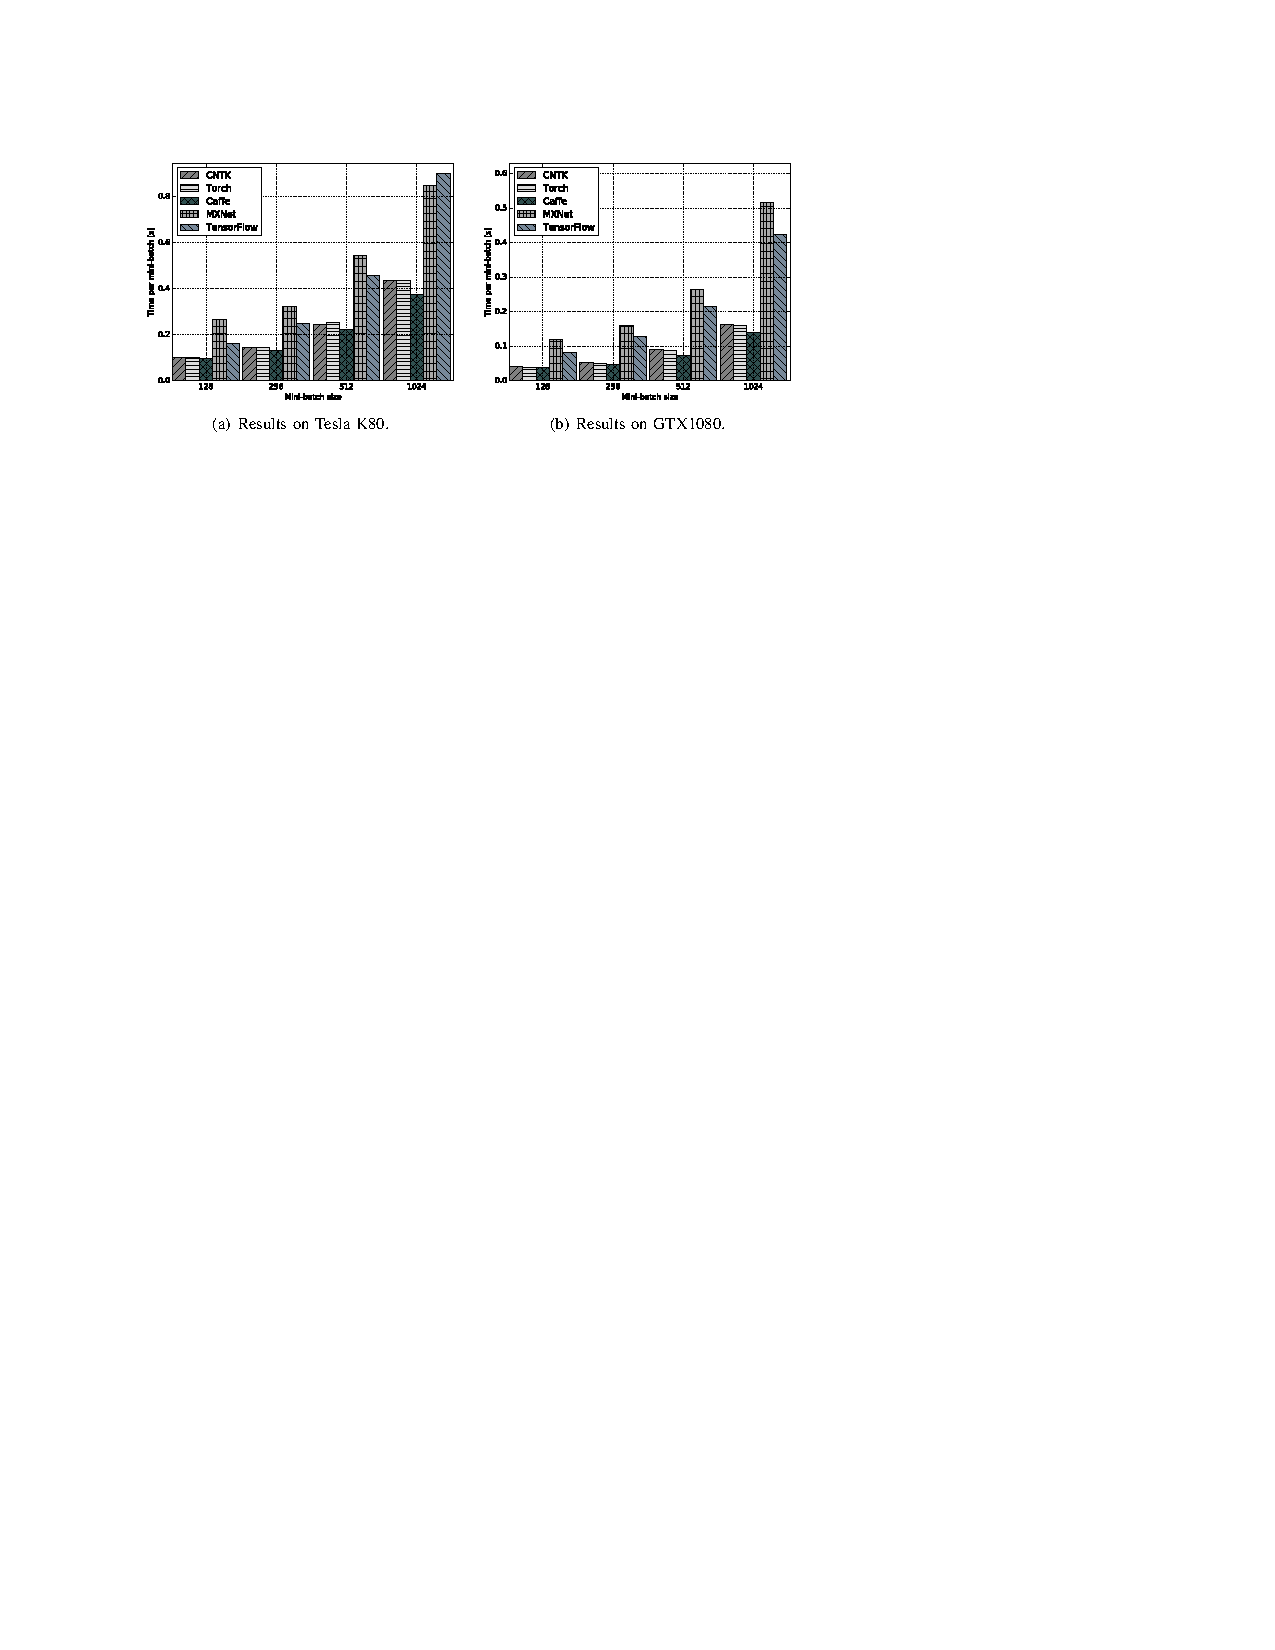
\includegraphics[width=\linewidth]{figures/FCN-S2.pdf} 
	\caption{The performance comparison of FCN-S on GPU platforms}
\end{figure}
%
\begin{figure}[htbp] 
	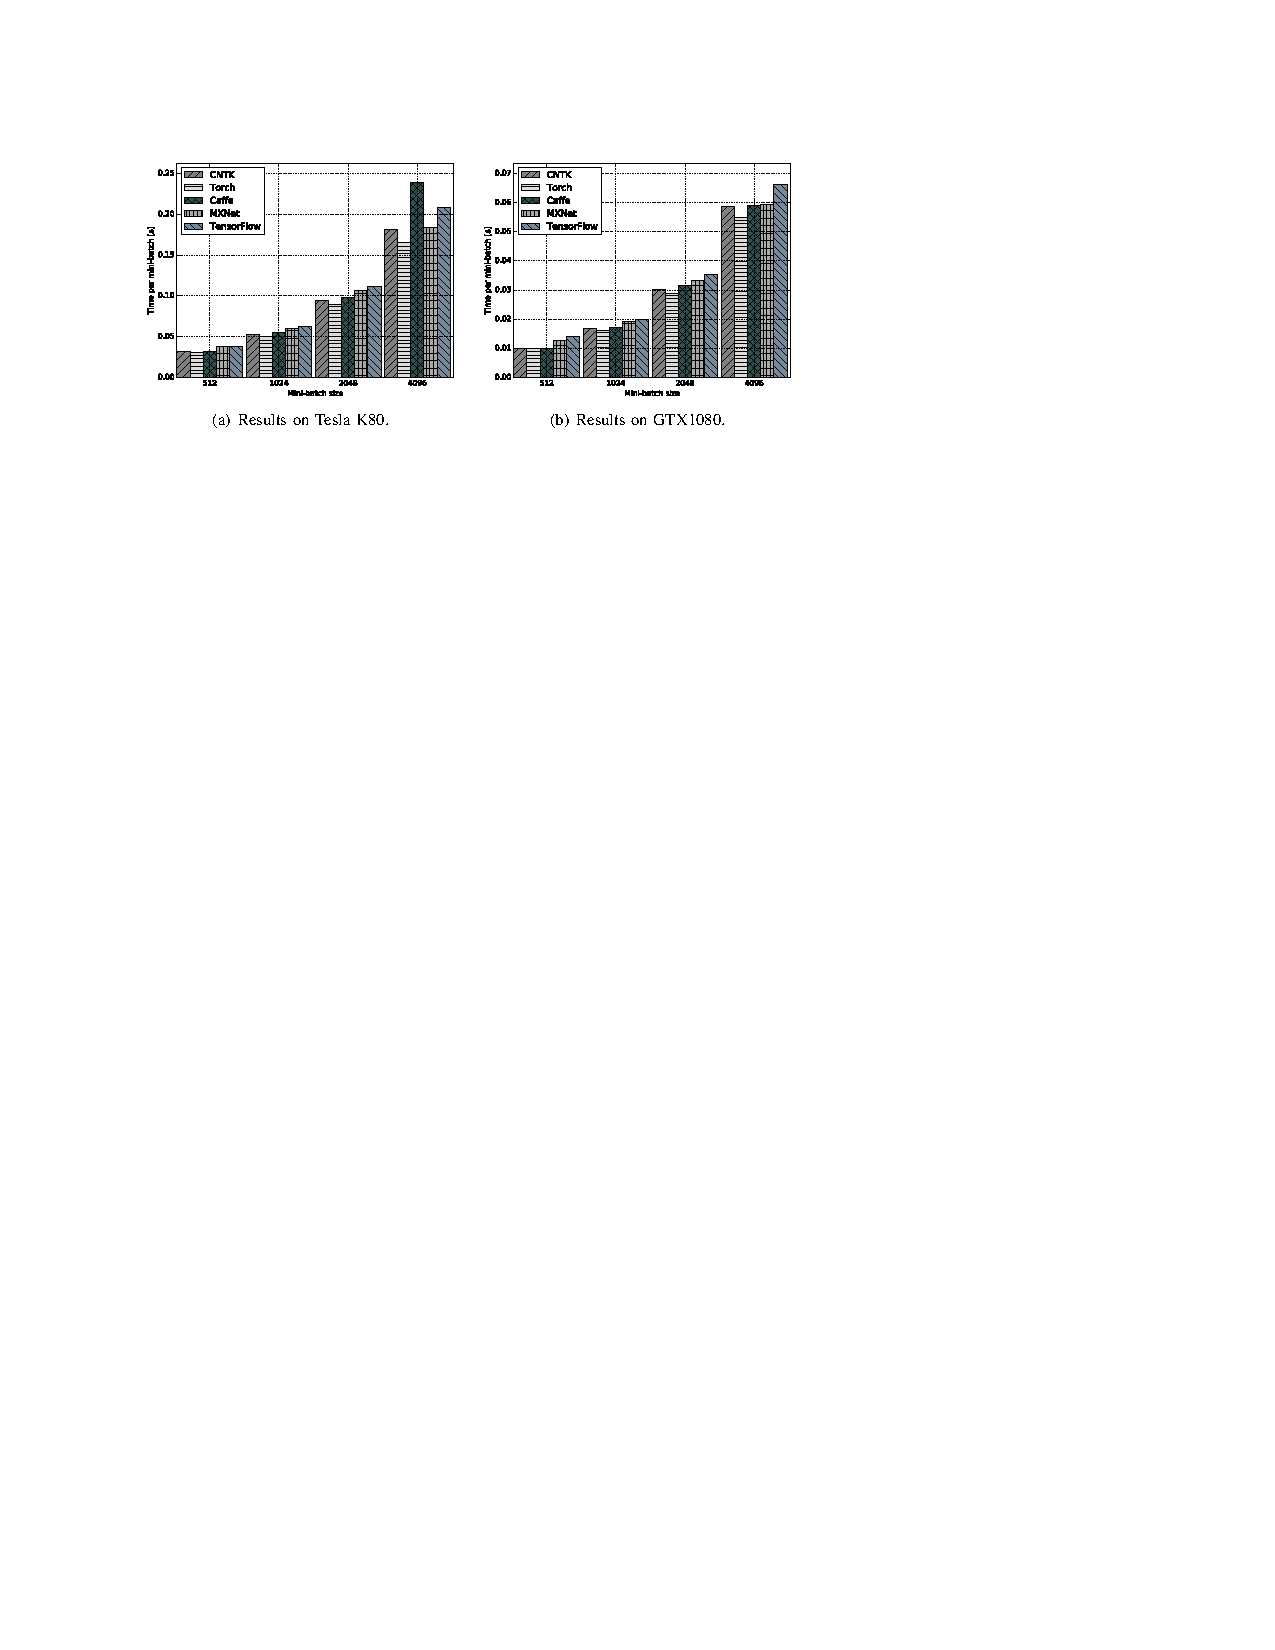
\includegraphics[width=\linewidth]{figures/FCN-R2.pdf} 
	\caption{The performance comparison of FCN-R on GPU platforms}
\end{figure}
%
\begin{figure}[htbp] 
	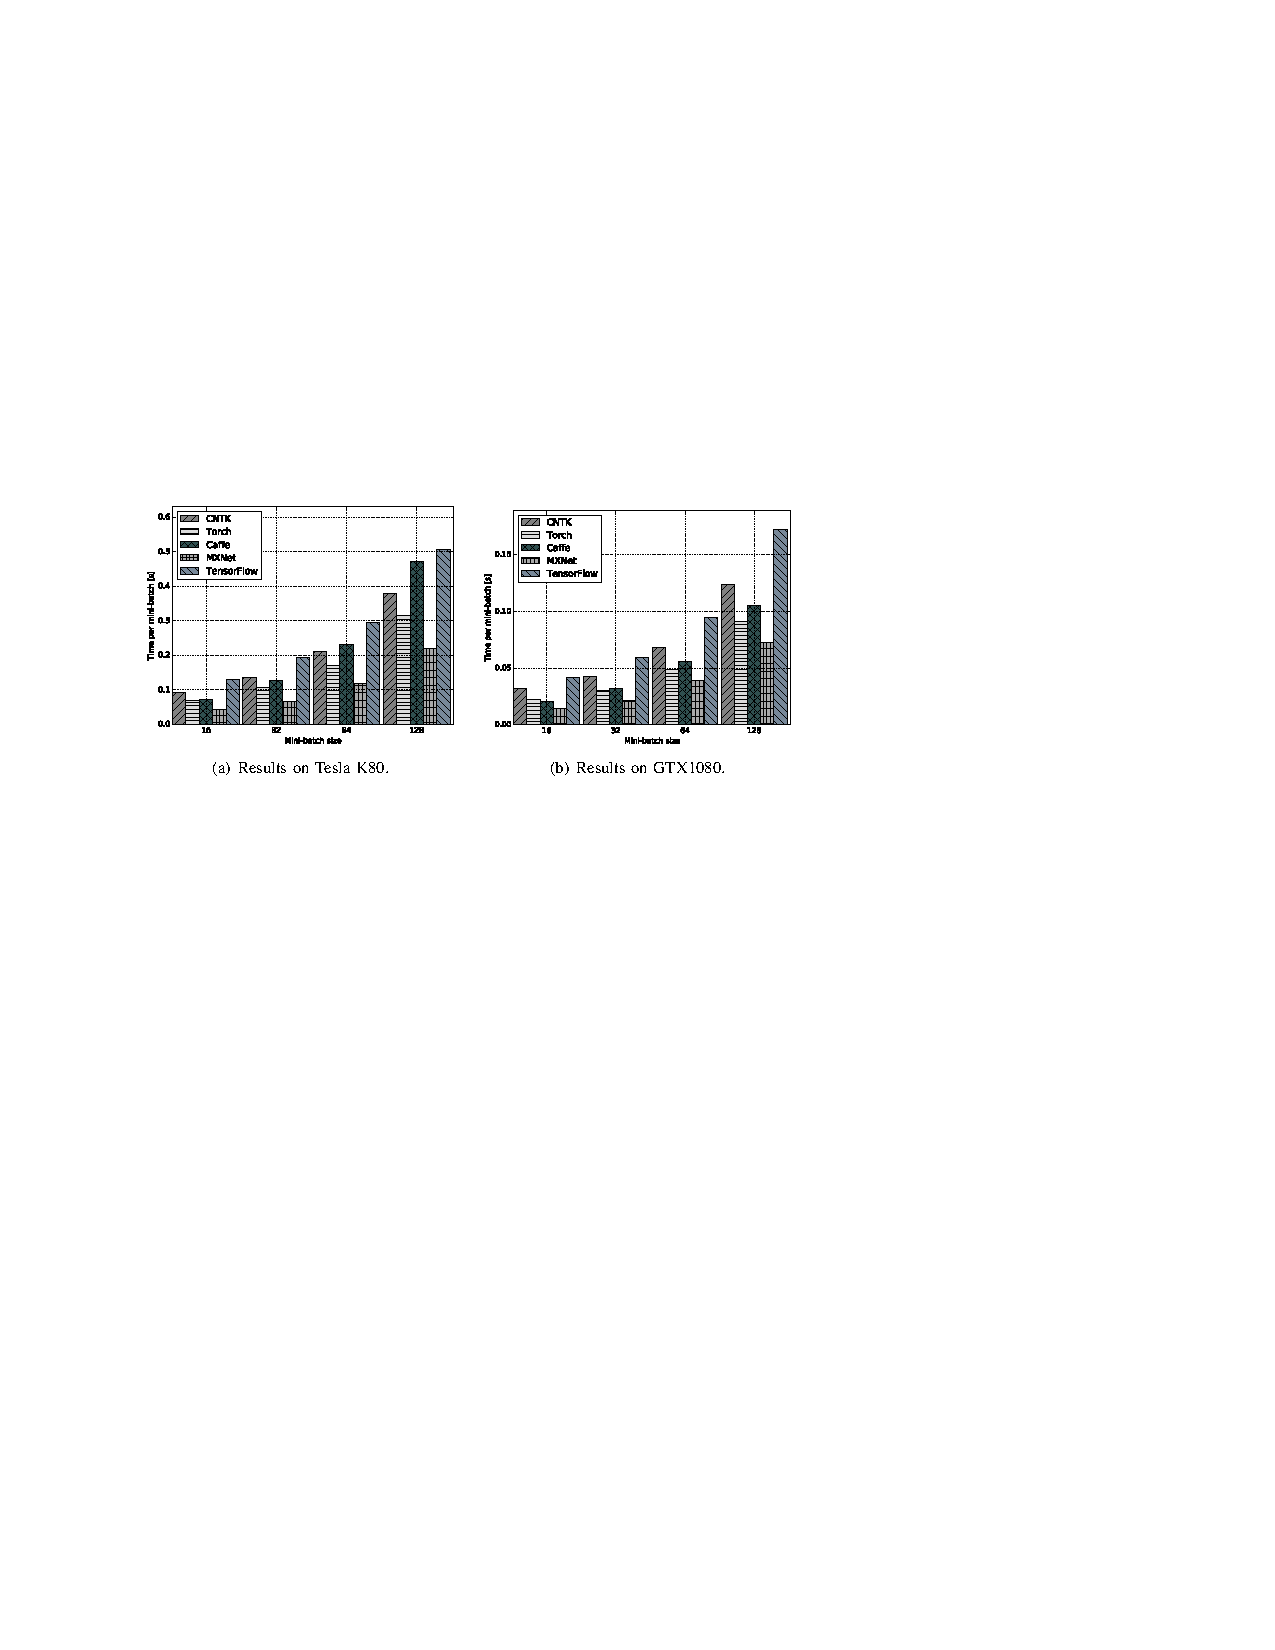
\includegraphics[width=\linewidth]{figures/AlexNet-S2.pdf} 
	\caption{The performance comparison of AlexNet-S on GPU platforms}
\end{figure}
%
\begin{figure}[htbp] 
	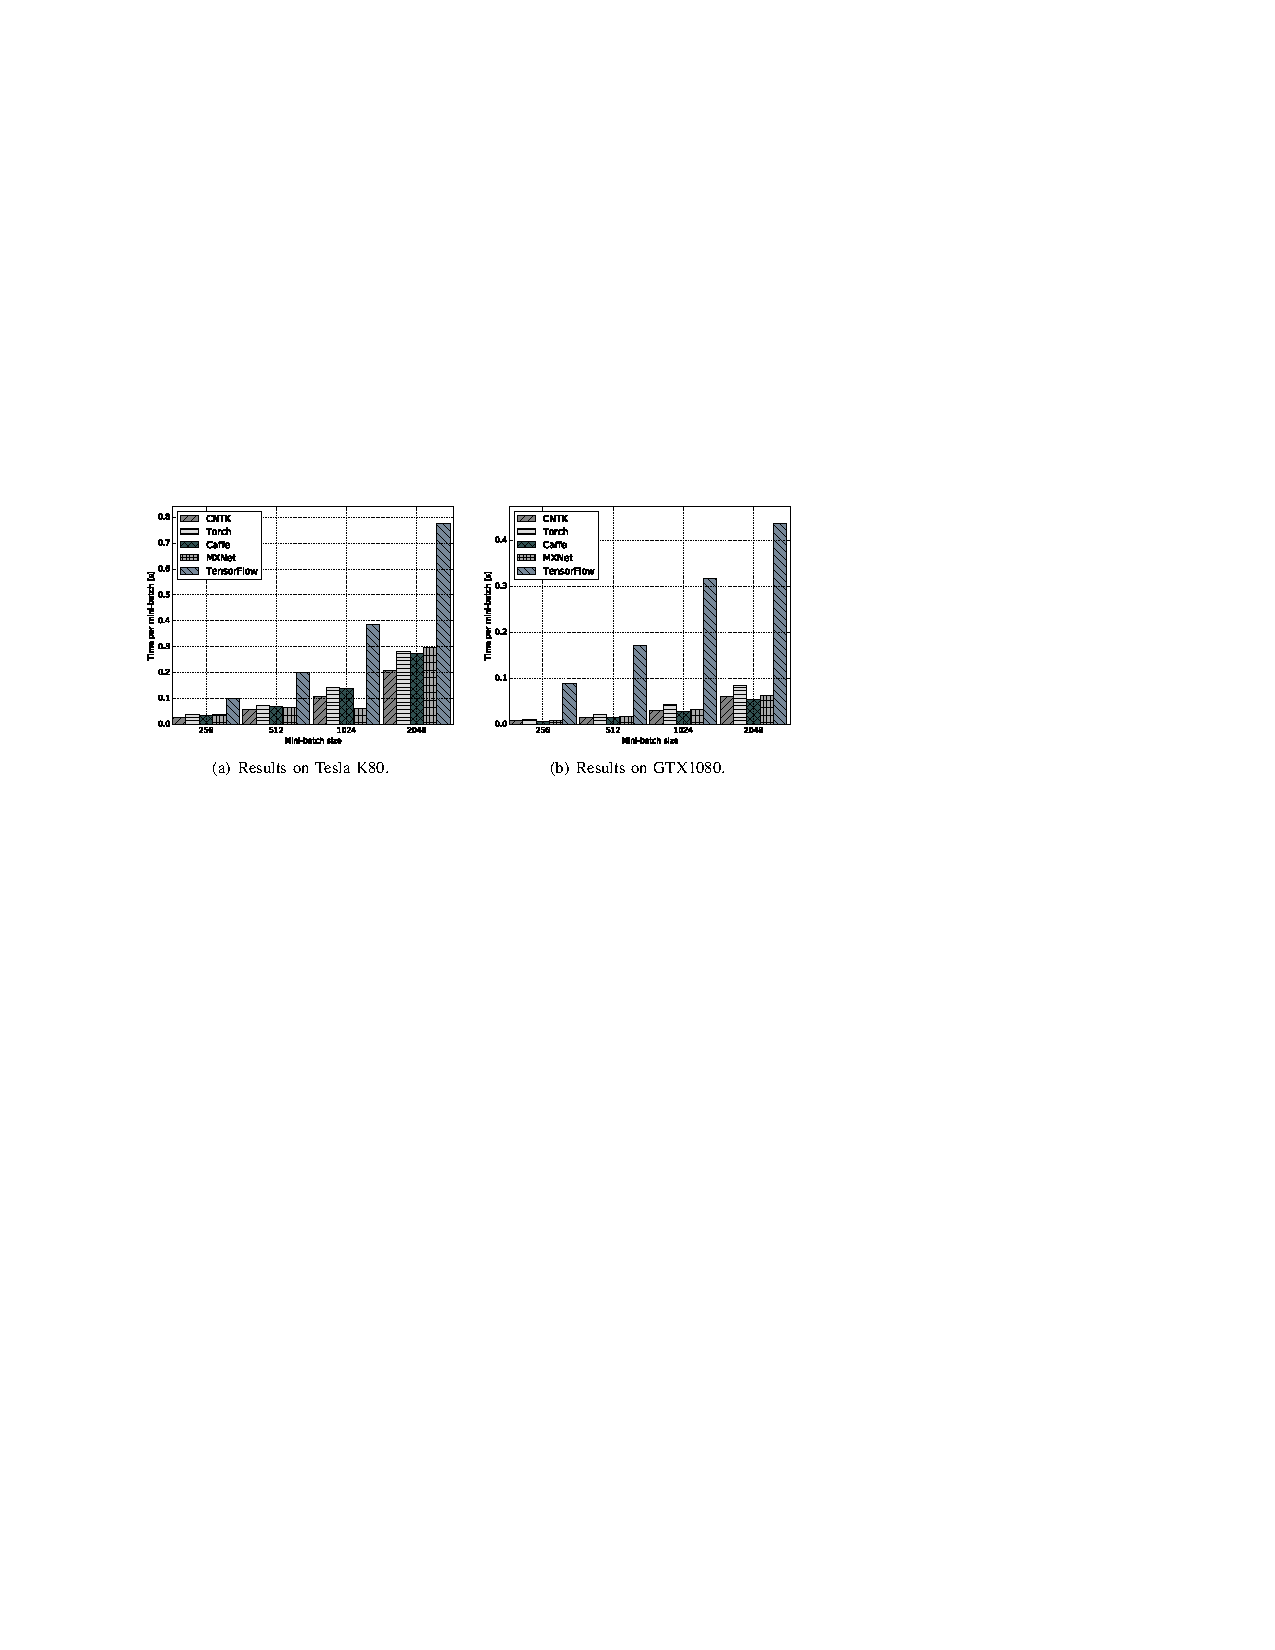
\includegraphics[width=\linewidth]{figures/AlexNet-R2.pdf} 
	\caption{The performance comparison of AlexNet-R on GPU platforms}
\end{figure}
%
\begin{figure}[htbp] 
	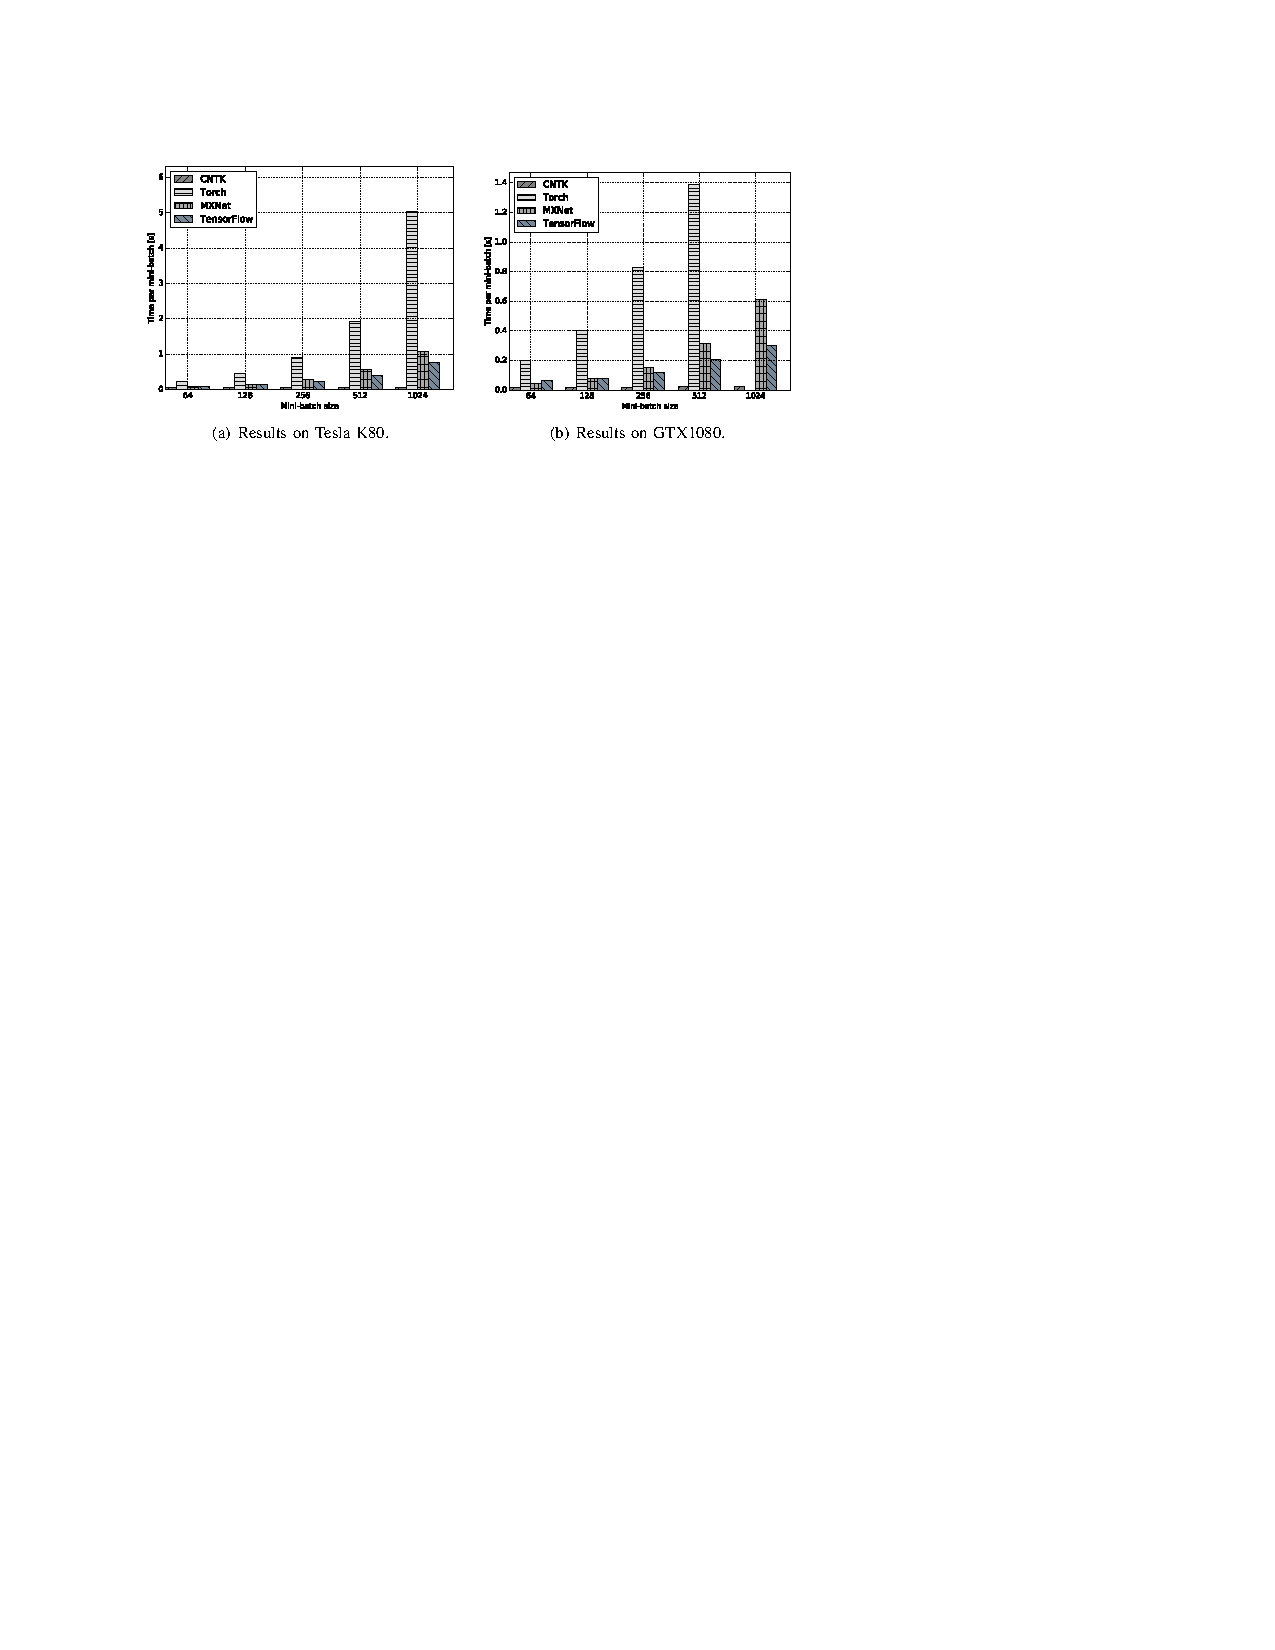
\includegraphics[width=\linewidth]{figures/LSTM2.pdf} 
	\caption{The performance comparison of LSTM on GPU platforms}
\end{figure}
%
\begin{figure}[!htbp]%[H]
\centering
\subfloat[Subfigure 1 list of figures text][FCN-R]{
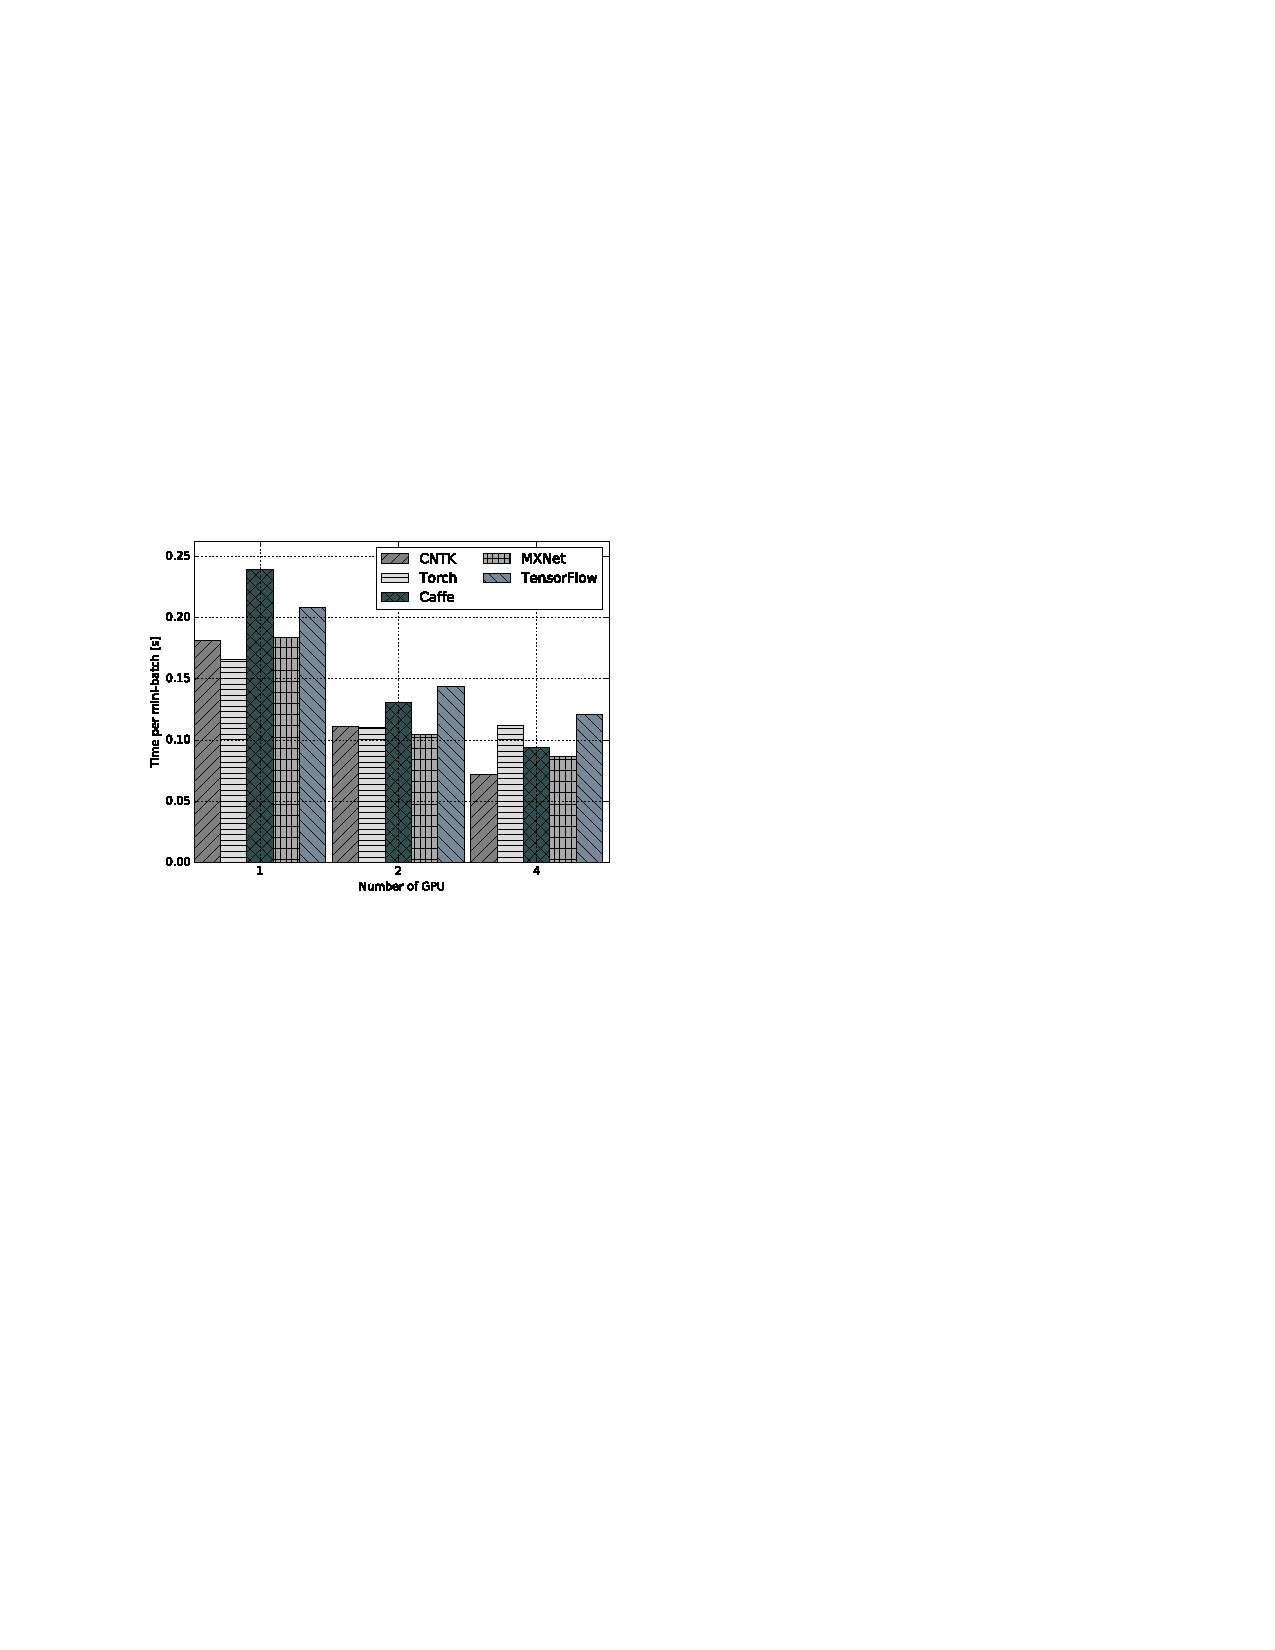
\includegraphics[width=0.48\textwidth]{figures/16a.pdf}
}
\subfloat[Subfigure 2 list of figures text][CNN-R]{
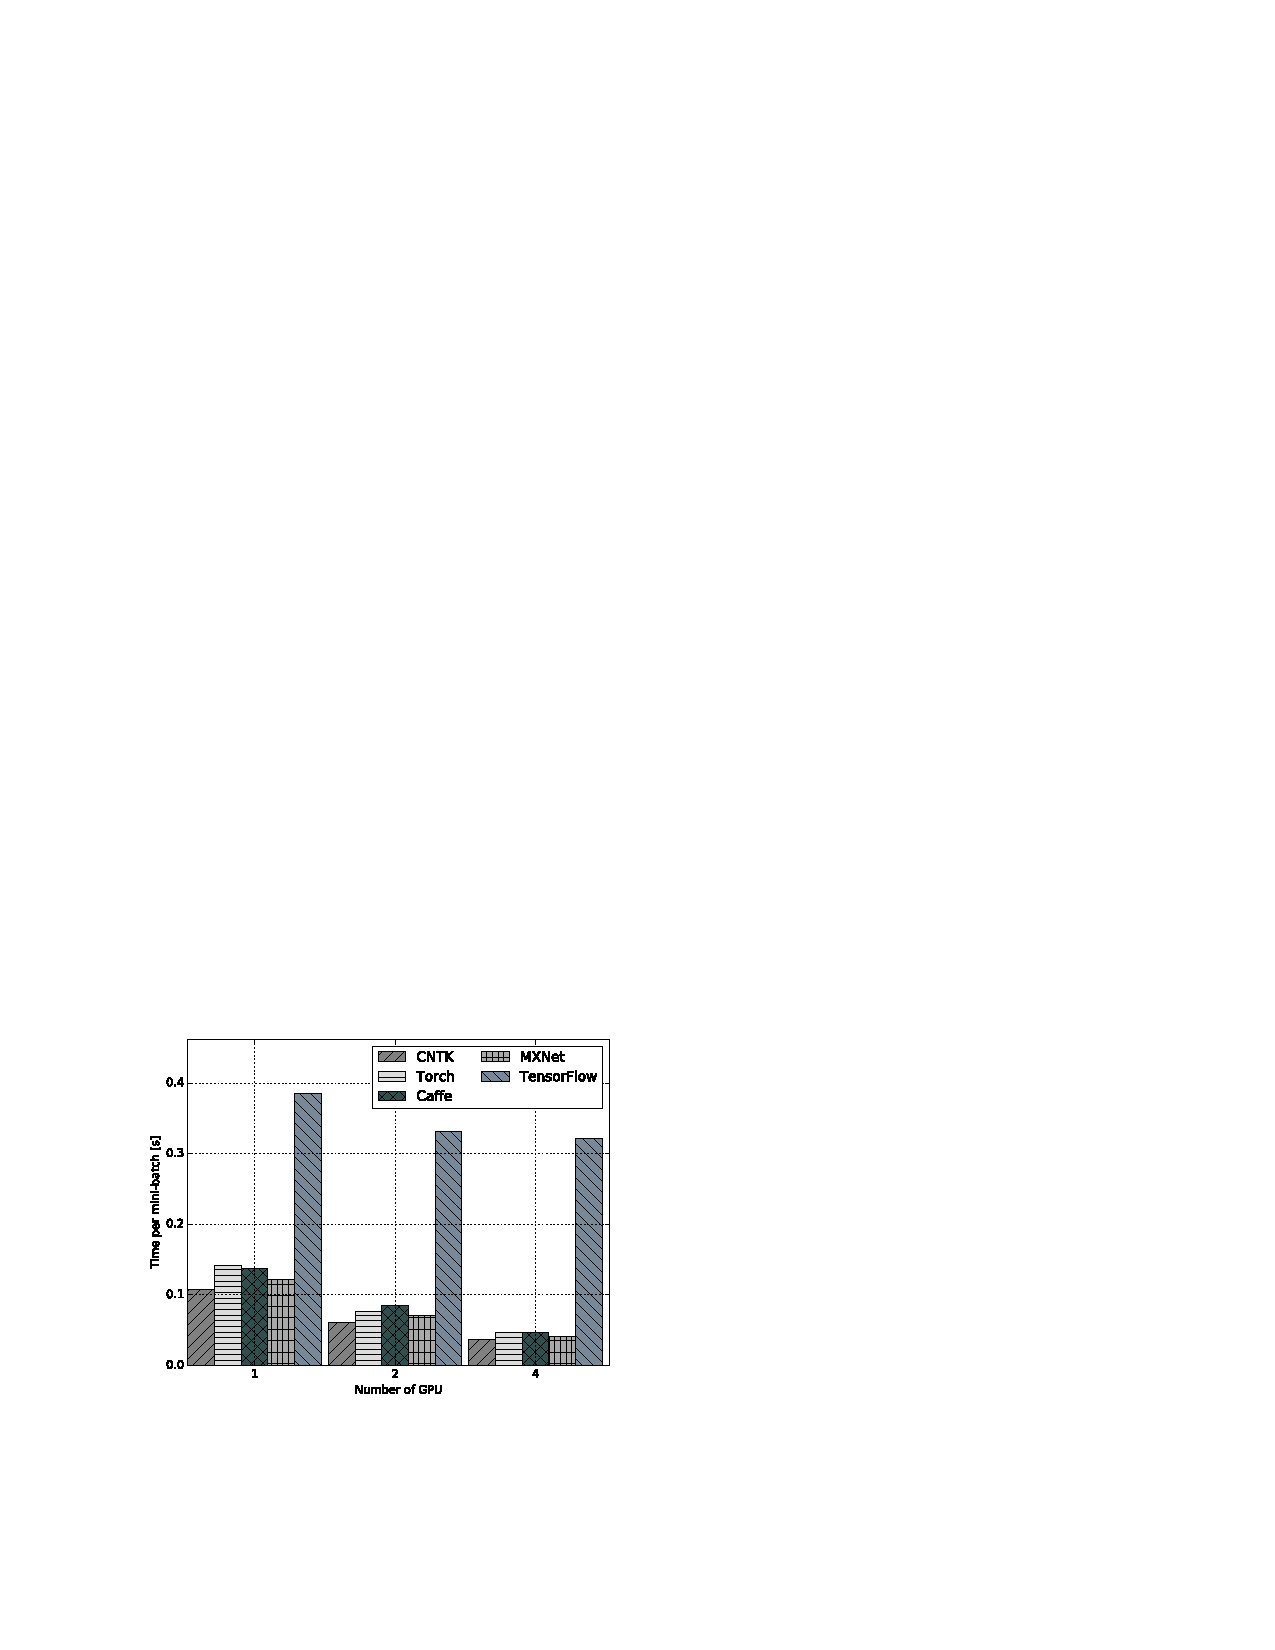
\includegraphics[width=0.48\textwidth]{figures/17a.pdf}
}
\caption{The scalability on a multi-GPU platform (2 $\times$ K80)}
\end{figure}

%%%
\section{TensorFlow}\label{sec:TF}
%%%

%%%
\subsection{Computational graph}
%%%

\begin{itemize}

\item Graph: In TensorFlow, ML algorithms are represented as computational graph. A computational graph (data flow graph) is a form of directed graph where vertices (nodes) describe operations, while edges represent data flowing between these operations.
	  	
\item Operation: An operation may represent a variable or constant, a control flow directive, a mathematical function, a file I/O, or a network communication port.
	  	
\item Tensor: A tensor is a multi-dimensional collection of homogeneous values with a fixed static type.
	  	
\item Variable: Variables can be described as persistent, mutable handles to in-memory buffers storing tensors.
	  	
\item Session: In TensorFlow the execution of operations and evaluation of tensors may only be preformed in a special environment called session.
	  	
\end{itemize}

%%%
\subsection{A simple example}
%%%

\begin{lstlisting}[language=python]
import tensorflow as tf

# Import training and test data from MNIST
import tensorflow.examples.tutorials.mnist.input_data as input_data
mnist = input_data.read_data_sets("MNIST_data/", one_hot=True)

graph = tf.Graph()

with graph.as_default():

    # Nodes can be grouped into visual blocks for TensorBoard
    with tf.name_scope('input_features'):
        x = tf.placeholder(tf.float32, shape=[None, 784], name='input_x')

    with tf.name_scope('input_labels'):
        y_ = tf.placeholder(tf.float32, shape=[None, 10], name='labels')

    with tf.name_scope('parameters'):
        W = tf.Variable(tf.zeros([784, 10]), name='weights')
        b = tf.Variable(tf.zeros([10]), name='biases')
        tf.summary.histogram('WEIGHTS', W)
        tf.summary.histogram('BIASES', b)
    
    with tf.name_scope('use_softmax'):
        y = tf.nn.softmax(tf.matmul(x, W) + b)

    with tf.name_scope('train'):
        # Compute the cross entropy of real label y_ and prediction label y
        cross_entropy = -tf.reduce_sum(y_*tf.log(y))
        # Create a gradient-descent optimizer with learning rate = 0.01
        train_step = tf.train.GradientDescentOptimizer(0.01).minimize(cross_entropy)

    with tf.name_scope('test'):
        correct_prediction = tf.equal(tf.argmax(y,1), tf.argmax(y_,1))
        accuracy = tf.reduce_mean(tf.cast(correct_prediction, "float"))
        # Track accuracy over time for TensorBoard
        tf.summary.scalar('Accuracy', accuracy)

    logpath = '/tmp/tensorboard'  # temporary path for storing TB summaries
    merged = tf.summary.merge_all()  # Merge all the summaries
    writer = tf.summary.FileWriter(logpath, graph)  # Write summaries

with tf.Session(graph=graph) as sess:
    # Initialize all variables
    tf.global_variables_initializer().run()
    
    for step in range(1,501):
        if (step%10) == 0:
            feed = {x: mnist.test.images, y_: mnist.test.labels}
            _, acc = sess.run([merged, accuracy], feed_dict=feed)
            print('Accuracy at %s step: %s' % (step, acc))
        else:
            batch_x, batch_y = mnist.train.next_batch(100)
            sess.run(train_step, feed_dict={x: batch_x, y_: batch_y})
            writer.add_summary(merged.eval(feed_dict={x: batch_x, y_: batch_y}), 
                               global_step=step)

    writer.close()

print("Run the command line to start TensorBoard:\n" \
      "(TensorFlow) $ tensorboard --logdir=/tmp/tensorboard" \
      "\nThen open http://0.0.0.0:6006/ into your web browser")
\end{lstlisting}

%%%
\section{MXNet}\label{sec:MxNet}
%%%

%%%
\subsection{Programming interface}
%%%

\begin{itemize}
%
\item Used to power Amazon Web Services (AWS)
%
\item Support many different applications (e.g. computer vision, natural language processing,  speech recognition, unsupervised machine learning, support embedded APIs, visualization)
%
\item Mixed programming style: imperative and declarative
\begin{itemize}
\item Light-weighted (around 50K lines of core code)
\item Data parallelism with multi-devices: 88\% scalability with 256 GPUs
\item Support many front-ends, including JavaScript (run on web browsers)
\item Provide intermediate-level and high-level interface modules
\item Provide abundant IO functions 
%
\end{itemize}
%
\item Fully compatible with Torch: modules and operators
%
\item Visualize neural network graphs
\begin{itemize}
\item Call mx.viz.plot\_network( )
\end{itemize}
%
\item Not well documented, code not easy to read
%
\end{itemize}

%%%
\subsection{A simple example}
%%%

\begin{lstlisting}[language=python]
import os, gzip, struct
import numpy as np
import mxnet as mx

# Read data from the MNIST dataset
def read_data(label_url, image_url):
    with gzip.open(label_url) as flbl:
        magic, num = struct.unpack(">II", flbl.read(8))
        label = np.fromstring(flbl.read(), dtype=np.int8)
    with gzip.open(image_url, 'rb') as fimg:
        magic, num, row, col = struct.unpack(">IIII", fimg.read(16))
        image = np.fromstring(fimg.read(),dtype=np.uint8).reshape(len(label),row,col)
    return (label, image)

train_lbl_file = 'train-labels-idx1-ubyte.gz'
train_img_file = 'train-images-idx3-ubyte.gz'
train_lbl, train_img = read_data(train_lbl_file, train_img_file)

test_lbl_file = 't10k-labels-idx1-ubyte.gz'
test_img_file = 't10k-images-idx3-ubyte.gz'
test_lbl,  test_img  = read_data(test_lbl_file, test_img_file)

# Create data iterators for MXNet
def to4d(img):
    return img.reshape(img.shape[0], 1, 28, 28).astype(np.float32)/255

batch_size = 100
train_iter = mx.io.NDArrayIter(to4d(train_img), train_lbl, batch_size, shuffle=True)
test_iter  = mx.io.NDArrayIter(to4d(test_img), test_lbl, batch_size)

# Define the network
data = mx.sym.Variable('data') # Create a place holder variable for the input data
data = mx.sym.Flatten(data=data)# Flatten the data from 4-D shape into 2-D
fc1  = mx.sym.FullyConnected(data=data, name='fc1', num_hidden=64) 
act1 = mx.sym.Activation(data=fc1, name='relu1', act_type="relu")
fc2  = mx.sym.FullyConnected(data=act1, name='fc2', num_hidden = 32)
act2 = mx.sym.Activation(data=fc2, name='relu2', act_type="relu")
fc3  = mx.sym.FullyConnected(data=act2, name='fc3', num_hidden=10)
out  = mx.sym.SoftmaxOutput(data=fc3, name='softmax')
mod  = mx.mod.Module(out)

# Plot the network graph
mx.viz.plot_network(symbol=out, shape={'data': (batch_size, 1, 28, 28)}).view()

# Prepare output log infomation
import logging
logging.getLogger().setLevel(logging.INFO)

# Train the network
mod.fit(train_data=train_iter, eval_data=test_iter, num_epoch=25)
\end{lstlisting}

\end{document}
